\documentclass[10pt,a4paper]{article}
\usepackage[utf8x]{inputenc}
\usepackage{ucs}
\usepackage[spanish]{babel}
\usepackage[left=2cm,top=4cm,right=2cm,bottom=3cm]{geometry} 
\usepackage{amsmath}
\usepackage{amsfonts}
\usepackage{amssymb}
\usepackage{dcolumn}
\usepackage{float}
\usepackage{graphicx}
\usepackage{ esint }
\usepackage{fancyhdr}
\usepackage{enumerate} 
\pagestyle{fancy}
\usepackage{tocbibind}
\usepackage{setspace}
\usepackage{parskip}
\usepackage[hidelinks]{hyperref}
\usepackage{listings} 
\usepackage[svgnames]{xcolor}


\definecolor{codegreen}{rgb}{0,0.6,0}
\definecolor{codegray}{rgb}{0.5,0.5,0.5}
\definecolor{codepurple}{rgb}{0.58,0,0.82}
\definecolor{backcolour}{rgb}{0.95,0.95,0.92}

\lstset{basicstyle=\ttfamily}
\lstdefinestyle{mystyle}{
	%backgroundcolor=\color{backcolour},   
	commentstyle=\color{codegreen},
	keywordstyle=\color{magenta},
	numberstyle=\tiny\color{codegray},
	stringstyle=\color{codepurple},
	breakatwhitespace=false,         
	breaklines=true,                 
	keepspaces=true,                 
	numbers=left,                    
	numbersep=5pt                  
}
\lstset{literate=
  {á}{{\'a}}1 {é}{{\'e}}1 {í}{{\'i}}1 {ó}{{\'o}}1 {ú}{{\'u}}1
  {Á}{{\'A}}1 {É}{{\'E}}1 {Í}{{\'I}}1 {Ó}{{\'O}}1 {Ú}{{\'U}}1
  {à}{{\`a}}1 {è}{{\`e}}1 {ì}{{\`i}}1 {ò}{{\`o}}1 {ù}{{\`u}}1
  {À}{{\`A}}1 {È}{{\'E}}1 {Ì}{{\`I}}1 {Ò}{{\`O}}1 {Ù}{{\`U}}1
  {ä}{{\"a}}1 {ë}{{\"e}}1 {ï}{{\"i}}1 {ö}{{\"o}}1 {ü}{{\"u}}1
  {Ä}{{\"A}}1 {Ë}{{\"E}}1 {Ï}{{\"I}}1 {Ö}{{\"O}}1 {Ü}{{\"U}}1
  {â}{{\^a}}1 {ê}{{\^e}}1 {î}{{\^i}}1 {ô}{{\^o}}1 {û}{{\^u}}1
  {Â}{{\^A}}1 {Ê}{{\^E}}1 {Î}{{\^I}}1 {Ô}{{\^O}}1 {Û}{{\^U}}1
  {œ}{{\oe}}1 {Œ}{{\OE}}1 {æ}{{\ae}}1 {Æ}{{\AE}}1 {ß}{{\ss}}1
  {ű}{{\H{u}}}1 {Ű}{{\H{U}}}1 {ő}{{\H{o}}}1 {Ő}{{\H{O}}}1
  {ç}{{\c c}}1 {Ç}{{\c C}}1 {ø}{{\o}}1 {å}{{\r a}}1 {Å}{{\r A}}1
  {€}{{\euro}}1 {£}{{\pounds}}1 {«}{{\guillemotleft}}1
  {»}{{\guillemotright}}1 {ñ}{{\~n}}1 {Ñ}{{\~N}}1 {¿}{{?`}}1
}

\lstset{showstringspaces=false}
\lstloadlanguages{C++}
\lstset{basicstyle=\ttfamily\footnotesize}
\lstset{style=mystyle}
\usepackage[titletoc,toc,page]{appendix}
\usepackage{pdfpages}
\renewcommand{\appendixtocname}{Anexo}
\renewcommand{\appendixpagename}{Anexo}
\lhead{Proyecto Final }
\rhead{
\includegraphics[width=1.5 cm]{logo}}
\author{cyn}
\begin{document}
\begin{titlepage}
\begin{center}
\vspace*{-1in}
\begin{figure}[htb]
\begin{flushleft}

\includegraphics[width=5cm]{./logo}
\end{flushleft}
\end{figure}
\begin{LARGE}
\textbf{U.B.A. FACULTAD DE INGENIERÍA}\\
\end{LARGE}
\vspace*{0.15in}
\begin{LARGE}
\textbf{Departamento de Electrónica}\\
\end{LARGE}
\vspace*{0.2in}
\begin{LARGE}
\textbf{Organización de computadoras 66-20}\\
\end{LARGE}
\vspace*{0.2in}
\begin{Large}
\textbf{TRABAJO PRÁCTICO \#0}\\
\end{Large}
\vspace*{0.2in}
\begin{LARGE}
\textit{Infraestructura básica }\\
\end{LARGE}
\vspace*{0.2in}
\begin{Large}
\raggedright\textbf{Curso: 2018 - 2do Cuatrimestre}\\
\end{Large}
\vspace*{0.1in}
\begin{Large}
\raggedright\textbf{Turno: Martes}\\
\end{Large}
\vspace*{0.1in}

\begin{table}[htb]
\begin{center}
\begin{spacing}{1.9}
\begin{tabular}{| l | l |}
\hline
\multicolumn{2}{|>{\arraybackslash}p{15cm}|}{\begin{Large}
\textbf{GRUPO N°}
\end{Large}}\\
\hline
\textbf{Integrantes} & \textbf{Padrón} \\
\hline
\makebox[8cm][c]{Verón, Lucas} & \makebox[2.5cm][c]{89341}\\
\hline
\makebox[8cm][c]{Gamarra Silva, Cynthia Marlene} & \makebox[2.5cm][c]{92702}\\
\hline
\makebox[8cm][c]{Gatti, Nicolás} & \makebox[2.5cm][c]{93570}\\
\hline
\textbf{Fecha de entrega: } & \hspace{0.8cm}23-11-2018\\
\hline
\textbf{Fecha de aprobación: } & \\
\hline
\textbf{Calificación: } & \\
\hline
\textbf{Firma de aprobación:} & \\
\hline
\end{tabular}
\end{spacing}
\end{center}
\end{table}
\fbox{%
\begin{minipage}[c][3.4cm][l]{.9\linewidth}
\textbf{Observaciones:} \\
\vfill
\end{minipage}
}
\end{center}

\vspace*{0.1in}
\end{titlepage}
\tableofcontents 
\vspace*{0.3in}
\newpage

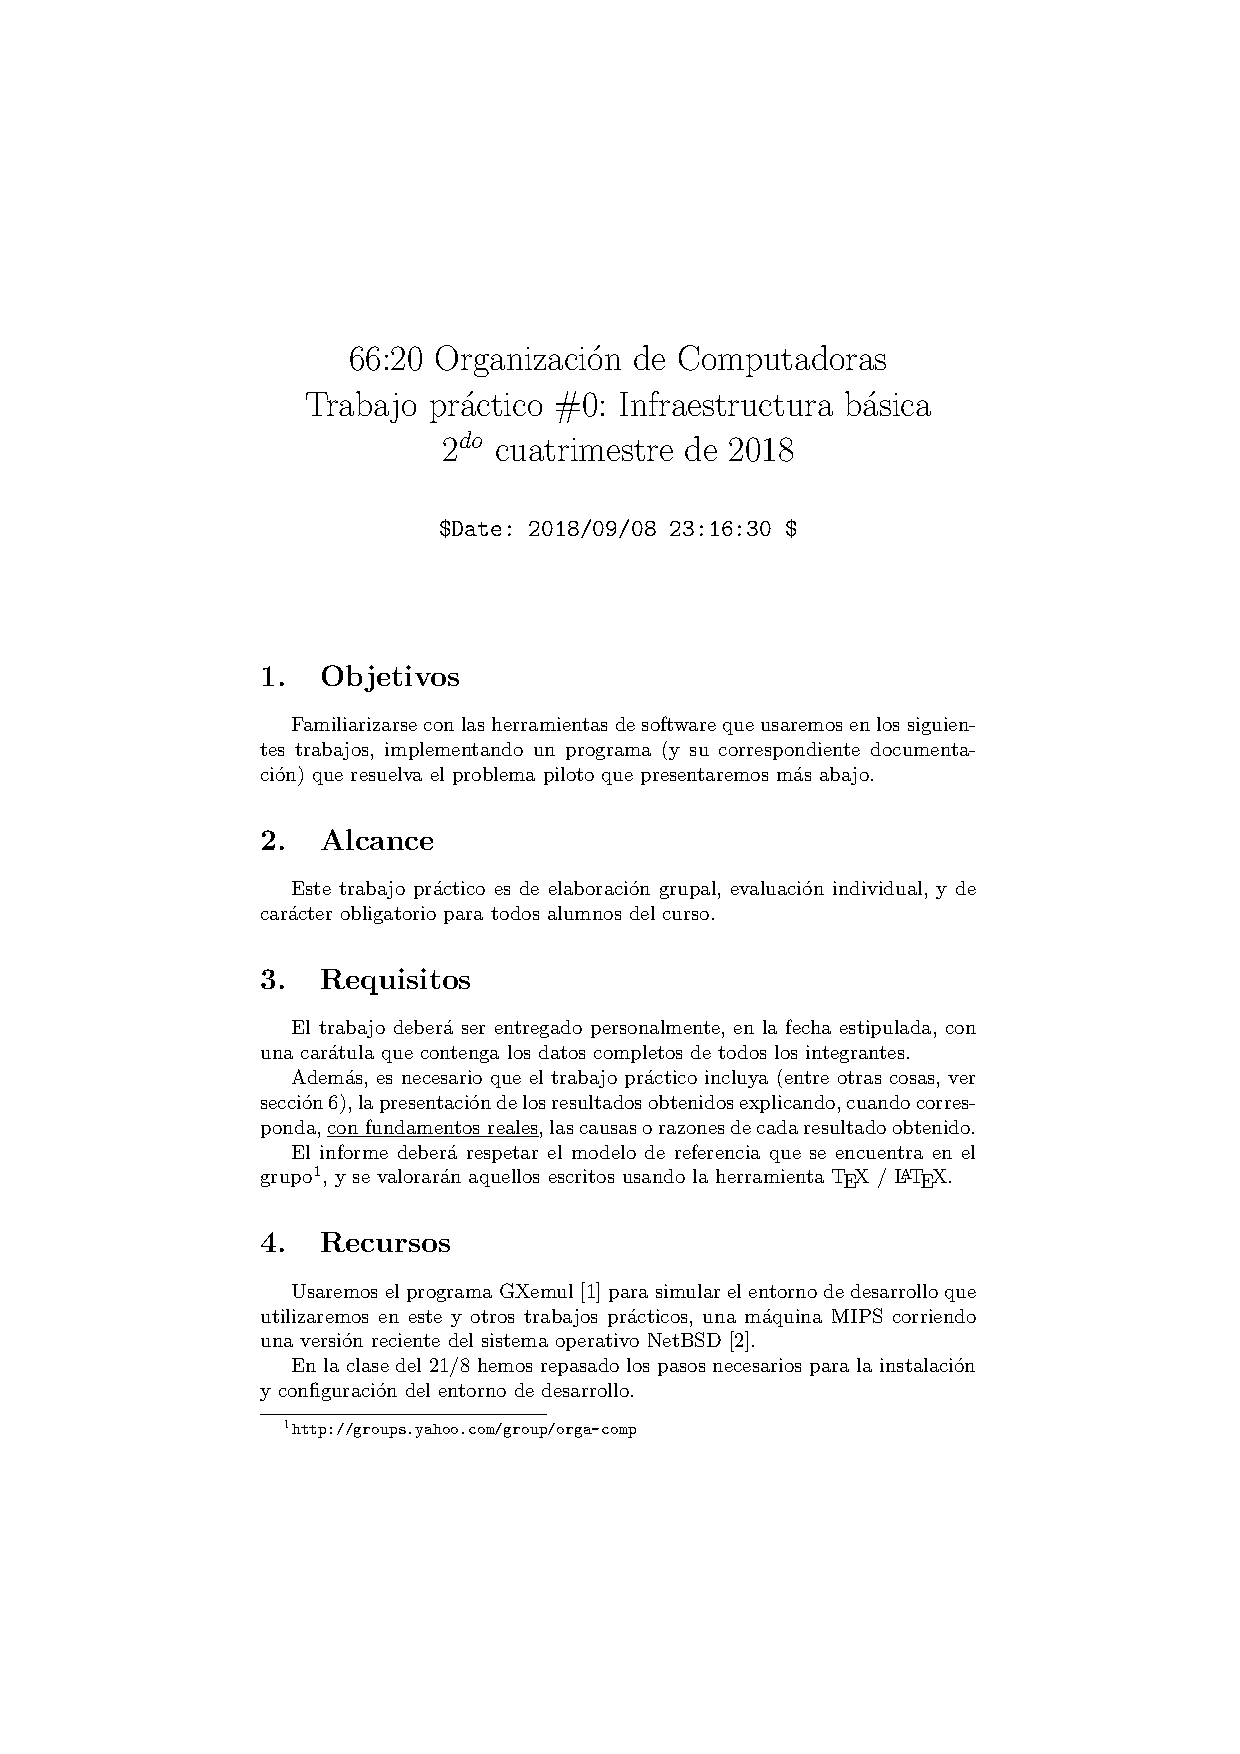
\includepdf[pages=1,scale=0.95,pagecommand = \section{Enunciado del trabajo práctico}\label{enunciado},offset=10 -10]{../tp0-2018-2q.pdf}
\includepdf[pages={2-last},scale=0.95,pagecommand = {},offset=10 -10]{../tp0-2018-2q.pdf}


\newpage

\subsection{Diseño e implementación}

El programa que contiene la lógica de codificador y decodificador se encuentra en el archivo \textit{\textbf{encode.c}}.
El codificador transforma expresiones con caracteres ASCII en base64, mientras que el decodificador hace el proceso inverso.
Ambas funciones se implementan con diversos ciclos y recorridos, así como utilización de instrucciones aritmético lógicas (sumas, \&, shifts, etc) que relacionan la codificación base 64 con ASCII.

Se creó un achivo \textit{\textbf{file.c}} para el manejo de los archivos a codificar/decodificar. Además se creó otro archivo llamado \textit{\textbf{command.c}} cuya función es tomar los parámetros del programa y realizar las acciones pertinentes a la misma. 

\newpage

\subsection{Parámetros del programa}

Se detallan a continuación los parámetros del programa

\begin{itemize}
    \item -h: Visualiza la ayuda del programa, en la que se indican los parámetros y sus objetivos.
    \item -V: Indica la versión del programa.
    \item -i: Archivo de entrada del programa.
    \item -o: Archivo de salida del programa.
    \item -a: Acción a llevar a cabo: codificación o decodificación.
\end{itemize}

Se indica a continuación detalles respecto a los parámetros:

\begin{itemize}
    \item Si no se explicitan -i y -o, se utilizarán stdin y stdout, respectivamente. 
    \item -V es una opción "show and quit ". Si se explicita este parámetro, sólo se imprimirá la versión, aunque el resto de los parámetros se hayan explicitado. 
    \item -h también es de tipo "show and quit" y se comporta de forma similar a -V.
    \item en caso de que se use la entrada estándar (con comando echo texto | ./tp0 etc) y luego se especifique un archivo de salida con -i, prevalecerá el establecido por parámetro.
\end{itemize}

\subsection{Compilación del programa}

La compilación del archivo fuente se realiza de la siguiente manera


\begin{lstlisting}
$ make
\end{lstlisting}


Para proceder a la ejecución del programa, se debe llamar a (según el nombre elegido al compilar):

\begin{lstlisting}
$ ./tp0
\end{lstlisting}

seguido de los parámetros que se desee modificar, los cuales se indicaron en la sección 1.2.

En caso de ser entrada estándar (stdin) se podrá ejecutar de la siguiente forma:

\begin{lstlisting}
$ echo texto | ./tp0
\end{lstlisting}

También en este caso, se indican a continuación los parámetros a usar.

\newpage

\section{Pruebas con archivo bash test.sh}
Se realizan corridas de prueba con el siguiente script

\begin{lstlisting}
    #!/bin/bash

    n=1
    while :; do
            head -c $n </dev/urandom >/tmp/in.bin;
            ./tp0 -a encode -i /tmp/in.bin -o /tmp/out.b64;
            ./tp0 -a decode -i /tmp/out.bin -o /tmp/out.bin;
            if diff /tmp/in.bin /tmp/out.bin; then :; else
                    echo ERROR: $n;
                    break;
            fi
            echo ok: $n;
            n="`expr $n + 1`";
            rm -f /tmp/in.bin /tmp/out.b64 /tmp/out.bin o;
    done

\end{lstlisting}

El cual no presenta errores en ninguna de las corridas llevadas a cabo.

\newpage

\section{Pruebas realizadas}

Todas las pruebas que se presentan a continuación, están codificadas en los archivos de prueba ***.txt de forma que puedan ejecutarse y comprobar los resultados obtenidos.

Se indicaran a continuación lo siguiente: comandos para ejecutarlas, líneas de código que las componen y resultado esperado.


\subsubsection{Generales}


\begin{itemize}
    \item Mensaje de ayuda\\
    
\begin{lstlisting}
$ ./tp0 -h  o ./tp0 --help

Options:
  -V, --version    Print version and quit.
  -h, --help       Print this information.
  -i, --input      Location of the input file.
  -o, --output     Location of the output file.
  -a, --action     Program action: encode (default) or decode.
Examples:
  tp0 -a encode -i ~/input -o ~/output
  tp0 -a decode


\end{lstlisting}     
     
	\item Mensaje de version\\

            \begin{lstlisting}
$ ./tp0 -V  o ./tp0 --version
Version: 0.1
             \end{lstlisting}  
         
         
    \item Archivo de entrada no válido
            \begin{lstlisting}
$ ./tp0 -i archivoInvalido.txt

File Open Error; No such file or directory

             \end{lstlisting}  

\end{itemize}

\newpage


\begin{thebibliography}{10}
	\bibitem{}Base64 (Wikipedia) http://en.wikipedia.org/wiki/Base64
	\bibitem{}The NetBSD project, http://www.netbsd.org/
	\bibitem{book_Cprogr} Kernighan, B. W. - Ritchie, D. M. - \emph{C Programming Language} - 2\textsuperscript{nd} edition - Prentice Hall - 1988.
	\bibitem{gnu_make} \emph{GNU Make} - \hyperlink{make}{https://www.gnu.org/software/make/}
	\bibitem{valgrind} \emph{Valgrind} - \hyperlink{valgrind}{http://valgrind.org/}

\end{thebibliography}

%-----------------------------------%
%									%
%			Seccion:Fuente			%
%									%
%-----------------------------------%
\appendix
\section{Código fuente}\label{appendix_codigo_fuente}

\subsubsection{main.c}\label{main}
\lstinputlisting[language=C]{../src/main.c}

\newpage

%\subsubsection{Assembly}\label{main}
 %\newpage


\end{document}
